\documentclass[slovak]{beamer}
\usetheme{beaver}

\usepackage[T1]{fontenc}
\usepackage[utf8]{inputenc}
\usepackage{graphicx}
%%XML highlight
\usepackage{listings}
\usepackage{color}
\definecolor{gray}{rgb}{0.4,0.4,0.4}
\definecolor{darkblue}{rgb}{0.0,0.0,0.6}
\definecolor{cyan}{rgb}{0.0,0.6,0.6}

\lstset{
  basicstyle=\ttfamily,
  columns=fullflexible,
  showstringspaces=false,
  commentstyle=\color{gray}\upshape
}

\lstdefinelanguage{XML}
{
  morestring=[b]",
  morestring=[s]{>}{<},
  morecomment=[s]{<?}{?>},
  morecomment=[s]{<!--}{-->},
  stringstyle=\color{black},
  identifierstyle=\color{darkblue},
  keywordstyle=\color{cyan},
  morekeywords={xmlns,version,type}% list your attributes here
}
%%end XML hightlight

\newcommand{\jl}{$\frac{}{}$} 

\title{Caver Analyst XML projekt}
\date{2014}
\author{
	Jan Štourač, Henrich Lauko, Jiří Novotný, Karel Kubíček
}


\begin{document}

\begin{frame}
	\titlepage
\end{frame}

\begin{frame}
\frametitle{Caver Analyst}
	
\includegraphics[width=\linewidth]{caver_start.jpg}
\end{frame}

\begin{frame}
\frametitle{Caver Analyst}
	\begin{itemize}
		\item bioinformatický nástroj určený pro analýzu tunelů v proteinech
		\item široké využití v komunitě biochemiků a proteinových inženýrů 
		\item grafická nadstavba výpočetního jádra Caver (Chovancová at el. 2012)
		\item vlastní vizualizační jádro
	\end{itemize}
\end{frame}

\begin{frame}
\frametitle{Caver Application}
	\begin{center}
		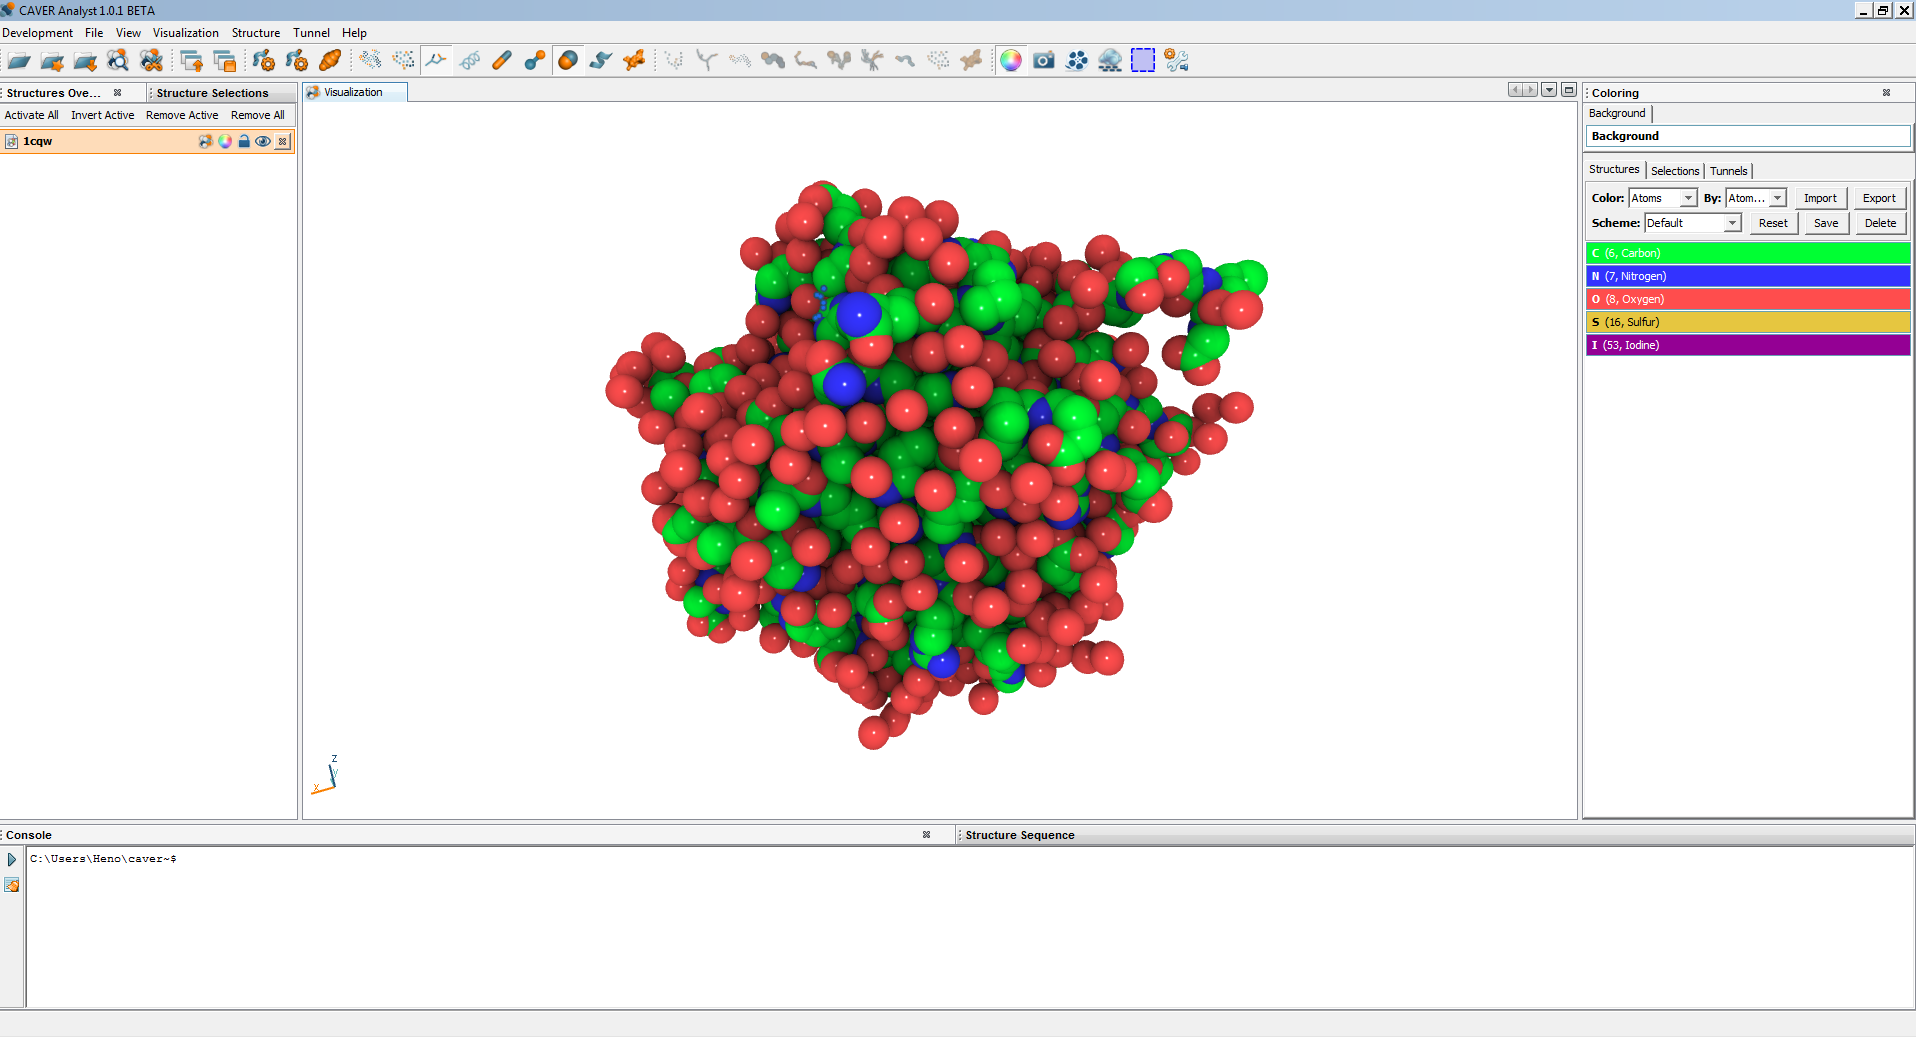
\includegraphics[width=\linewidth]{caver.png}
	\end{center}
\end{frame}

\begin{frame}
\frametitle{Cíle}
	\begin{itemize}
		\item uživatelská barevná schémata
		\begin{itemize}
			\item efektivní ukládání schémat do XML souboru
			\item podpora importu a exportu
			\item přívětivé uživatelské rozhraní
		\end{itemize}
		\item úprava XML s globálním nastavením aplikace
	\end{itemize}
\end{frame}

\begin{frame}
\frametitle{Organizace projektu}
	\begin{itemize}
		\item Rozdělení úloh:
		\begin{itemize}
			\item Backend - Jan Štourač
			\item GUI - Henrich Lauko
			\item XML struktura a XSD - Karel Kubíček
			\item Globální nastavení - Jiří Novotný
		\end{itemize}
		\item Využití interního svn repozitáře pro zdrojový kód
		\item Wiki na github.com
		\begin{itemize}
			\item Zakomponováno do interní dokumentace
		\end{itemize}
		\item kód dokumentován pomocí JavaDoc
	\end{itemize}
\end{frame}

\begin{frame}
\frametitle{Proces vývoje}
	\begin{itemize}
		\item 21. 3. - střetnutí o možnostech práce na projektu Caver a rozdělení úloh
		\item 22.3. - 20.4. - zorientovaní se v Caveru a práce na vývoji
		\item 21.4. - 4.5. - testovaní a drobné úpravy
		\item 5.4. - 22.5. - rozpracovaná verze dokumentace
		\item 22.5. - finalizace a prezentace projektu
	\end{itemize}
\end{frame}

\begin{frame}
\frametitle{Backend}
	\begin{itemize}
		\item návrh a implementace API pro práci s barevnými schématy
		\begin{itemize}
			\item globální manažer schémat pro celou aplikaci
		\end{itemize}
		\item oddělení systémových a uživatelských schémat
		\item notifikace o GUI při změnách
	\end{itemize}
\end{frame}

\begin{frame}
\frametitle{XML color schéma}
	\begin{itemize}
		\item návrh reprezentace barevných schémat v XML
		\item rozdělení default a user schémat
		\item ukládání schémat pomocí rozdílů
		\item kontrolní XSD schéma
		\item synchronizace schémat přes projektovou stránku
	\end{itemize}
\end{frame}

\begin{frame}[fragile]
\frametitle{XML color schéma}
	\lstset{language=XML}
	\scriptsize{
	\begin{lstlisting}
<?xml version="1.0" encoding="UTF-8"?>
<!--
    Document   : colorSchemes.xml
    Description: Native color schemes.
-->
<root xsi:noNamespaceSchemaLocation="company.xsd">
    <scheme type="Atoms" strategy="Atom element" name="Default">
        <color id="1" R="0.900" G="0.900" B="0.900"/>
        <color id="2" R="0.851" G="1.000" B="1.000"/>
    </scheme>
    <scheme type="Residues" strategy="Residue type" name="Default" >  
    </scheme>
    <scheme type="Chains" strategy="Chain identifier" name="Default" >
    </scheme>
    <scheme type="Secondary structures" 
	        strategy="Secondary structure type" name="CMY">
    </scheme>
</root>
	\end{lstlisting}}
\end{frame}

\begin{frame}
\frametitle{Color schémy GUI}
	\begin{itemize}
		\item návrh panelů pro práci so schémami
		\begin{itemize}
			\item možnosti spravování schémat
			\item panely pro import/export uživatelských schémat
		\end{itemize}
		\item rozdělení panelů do default a user profilů
		\item vyřešen problém synchronizace všech panelů pracujících s barevnými schématy
		\item možnost rozšiřování o další barevné strategie
	\end{itemize}
\end{frame}

\begin{frame}
\frametitle{Color schémy GUI}
	\frametitle{Color schémy GUI}
	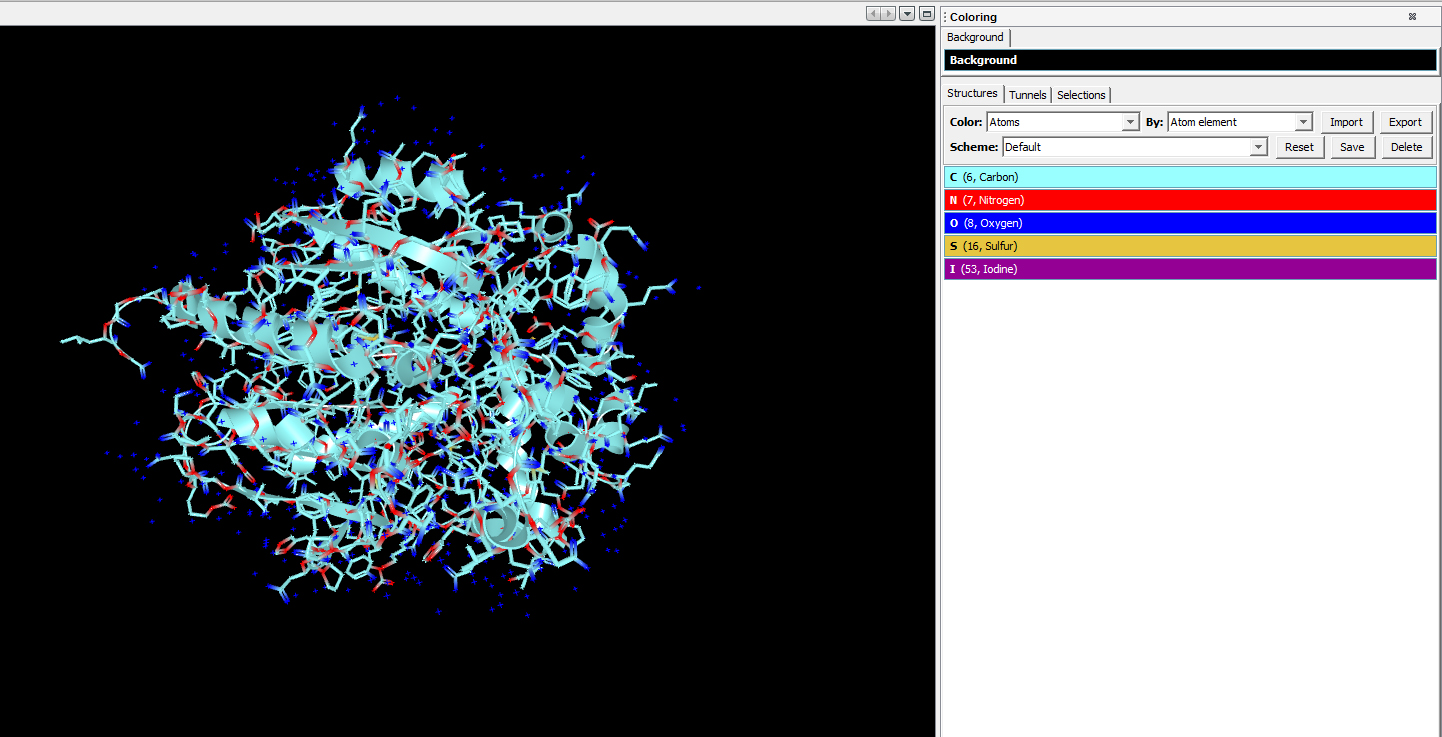
\includegraphics[width=\linewidth]{colorpanel.jpg}
\end{frame}

\begin{frame}
\frametitle{Global settings}
	\begin{itemize}
		\item nastavení uloženo v settings.xml v user home složce
		\item bugfix - nechtěné přepisování parametrů v nastavení při inicializaci programu
		\item bugfix - znaková sada settings.xml
		\item manuální editace souboru s nastavením => tvorba jeho XSD pro validaci
		\item restrukturalizace settings.xml pro podporu XSD validace
	\end{itemize}
\end{frame}

\begin{frame}[fragile]
	\frametitle{XML settings}
	\lstset{language=XML}
	\scriptsize{
	\begin{lstlisting}
<?xml version="1.0" encoding="UTF-8"?>
<!--
    Document   : settings.xml
    Description: Global settings of Caver Analyst
-->
<configuration>
  <entry key="CAVER_LOCALE">
    <locale>en_US</locale>
  </entry>
  <entry key="INTERPOLATE_DYNAMICS_TUNNELS">
    <boolean>false</boolean>
  </entry>
  <entry key="CAVER_COLORS_DIR">
    <string>C:\Users\Tracko\caver\colors</string>
  </entry>
</configuration>
	\end{lstlisting}}
\end{frame}

\begin{frame}
\frametitle{Zhodnocení projektu}
	\begin{itemize}
		\item vylepšená podpora barevných schémat
		\item možnost importu a exportu uživatelsky definovaných schémat
		\item zpřístupnění XSD souboru pro manuální validaci
		\item nové přívětivé uživatelské rozhraní
		\item snadná rozšiřitelnost aplikace o další barvitelné prvky
		\begin{itemize}
			\item jednoduše využitelné veřejné API
			\item notifikace jednotlivých komponent
		\end{itemize}
		\item vylepšená správa globálního nastavení aplikace 
	\end{itemize}
\end{frame}

\end{document}
